%%%%%%%%%%%%%%%%%%%%%%%%%%%%%%%%%%%%%%%%%%%%%%%%%%%%%%%%%%%%%%%%%%%%%%%%%%%%%%%%

\section{Analýza problému}
\label{sec_problem_analysis}

Použitá technika rozpoznávání aplikací v~šifrovaném TLS provozu využívá tzv. JA3 otisky (\textit{fingerprints}). Ty byly představeny pány John B. Althouse, Jeff Atkinson a Josh Atkins v~roce 2015.\footnote{\url{https://github.com/salesforce/ja3}} Technika spočívá v~tom, že ze síťové komunikace jsou vyfiltrovány TLS \textit{handshake} packety. Z~packetů \textit{Client Hello} a \textit{Server Hello} jsou vyextrahovány následující položky: \textit{Handshake Version}, \textit{Cipher Suites}, \textit{Extensions}, \textit{Supported Groups} a \textit{Elliptic Curve Point Format}. Z~těchto informací je spočítán MD5 hash (\textit{Message-Digest algorithm})~--~JA3 otisk.

\begin{figure}[H]
    \centering
    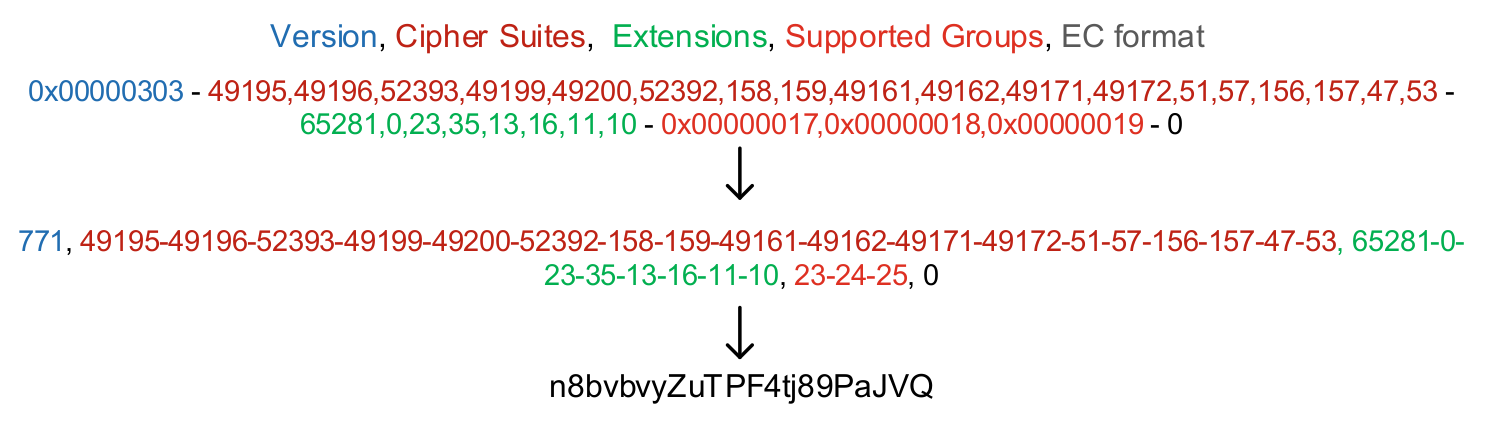
\includegraphics[width=0.99\linewidth]{ja3.png}
    \caption{Vytvoření JA3 otisku. Obrázek je převzatý~\cite{bib_matousek}.}
    \label{fig_ja3}
\end{figure}

Limitace tohoto řešení spočívá v~poměrně nízkém počtu možných otisků. Možností ustanovení TLS spojení není příliš velké. Porovnáváním pouze JA3 otisku pro danou aplikaci by nebylo dostatečné. Pravděpodobně pokud dvě aplikace využívají stejnou TLS knihovnu, jejich otisk bude stejný. Proto jako příznak pro rozpoznávání je třeba využít více informací, například SNI (\textit{Server Name Indication}).

%%%%%%%%%%%%%%%%%%%%%%%%%%%%%%%%%%%%%%%%%%%%%%%%%%%%%%%%%%%%%%%%%%%%%%%%%%%%%%%%
